\documentclass[twocolumn,floatfix,aps,prd,nofootinbib]{revtex4-2}

% Engine guard: glyphtounicode and \pdfgentounicode are pdfTeX primitives.
% Under LuaLaTeX/XeLaTeX they are undefined, the run aborts in the preamble,
% and every \cite comes out as "??".  LuaTeX and XeTeX emit correct ToUnicode
% maps on their own, so the block is simply skipped there.
\usepackage{iftex}
\ifPDFTeX
  \usepackage[utf8]{inputenc}
  \usepackage[T1]{fontenc}
  \usepackage{lmodern}
  \input{glyphtounicode}
  \pdfgentounicode=1
\else
  \usepackage{fontspec}
  \setmainfont{Latin Modern Roman}
  \setsansfont{Latin Modern Sans}
  \setmonofont{Latin Modern Mono}
\fi
\usepackage{graphicx}
\usepackage{amssymb}
\usepackage{amsmath}
\usepackage{xcolor}
\usepackage{hyperref}
\usepackage{textcase}
\usepackage{placeins}
\usepackage[protrusion=true,expansion=false]{microtype}

\graphicspath{{figures/}}

\hypersetup{
    colorlinks=true,
    linkcolor=blue,
    filecolor=magenta,
    urlcolor=blue,
    citecolor=blue,
}
\urlstyle{same}
\emergencystretch=2em

\begin{document}

\title{The Bondi dipole in full numerical relativity: a self-accelerating positive--negative mass binary}

\author{Nikita M. Shirokov}
\email{shirokov.nm@phystech.edu}
\affiliation{\textit{Moscow Institute of Physics and Technology, Moscow, Russia}}
\author{Ilya Nachevsky}
\email{ommnammashivaya@gmail.com}
\affiliation{\textit{Higher School of Economics, Moscow, Russia}}
\date{\today}

\begin{abstract}
Bondi showed in 1957 that a body of negative active gravitational mass, paired with a positive one, should accelerate together with it indefinitely while the total momentum stays zero. We test this prediction in full $3{+}1$ numerical relativity. The matter consists of two complex scalar fields with identical self-interactions. One of them enters the Einstein equations with the opposite sign, so its inertial and passive masses are positive and its active mass, and with it its Arnowitt--Deser--Misner (ADM) mass, is negative. We construct constraint-satisfying initial data for solitonic boson stars of both signs and run 34 simulations, including same-sign pairs and isolated stars as controls. A pair of stars with equal ADM mass magnitude, released from rest, accelerates as a single object at constant separation, while its total signed matter momentum stays zero to within 1\%. The acceleration scales with separation and mass as Bondi's Newtonian law predicts, reverses when the two stars are exchanged, and is absent in every control. We detect no gravitational radiation from the accelerating pair, consistent with the absence of a mass dipole. To our knowledge, the negative-mass star is the first asymptotically flat body of negative ADM mass evolved in numerical relativity. Our simulations cover head-on pairs released from rest and followed up to a few percent of the speed of light.
\end{abstract}

\maketitle

\section{Introduction}
\label{sec:intro}

Bondi~\cite{bondi1957} distinguished three kinds of mass in general relativity: the inertial mass, which resists acceleration; the passive gravitational mass, on which a gravitational field acts; and the active gravitational mass, which sources the field. He showed that a body whose active mass alone is negative is attracted by a positive mass, while the positive mass is pushed away from it. Released together, the two accelerate in the same direction without limit (Fig.~\ref{fig:schematic}), and momentum is conserved because the negative body's momentum counts with a negative sign. Bonnor and Swaminarayan~\cite{bonnor_swami1964} found exact solutions for uniformly accelerated pairs of this kind, later generalized in Ref.~\cite{bicak1983}. Forward~\cite{forward1990} showed that the self-accelerating pair conserves both momentum and energy, for equal and unequal mass magnitudes, so objections to negative mass must rest on other grounds~\cite{hoffmann1966,martins1980}. Newtonian $N$-body simulations have since applied the same sign rules to cosmological structure formation~\cite{manfredi2018,manfredi2026}.

\begin{figure}[t]
\centering
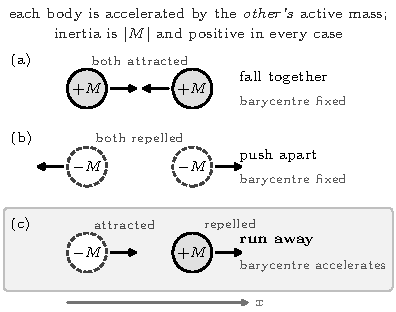
\includegraphics{fig_schematic.pdf}
\caption{Bondi's sign rules for two bodies released from rest, after Forward~\cite{forward1990}. Every body has positive inertial and passive mass; the active mass of the dashed bodies is negative. (a)~Two positive masses attract and (b)~two negative masses repel; in both cases the forces are opposite and the barycentre stays at rest. (c)~For a positive and a negative mass both forces point the same way, so the pair accelerates while its total momentum stays zero.}
\label{fig:schematic}
\end{figure}

Nothing in the Einstein equations requires mass to be positive. Positivity of the total mass is a theorem only for matter that satisfies energy conditions~\cite{schoen_yau1979,witten1981}, and several candidate sources violate them: Casimir energies, quantum fields in curved spacetime and phantom dark energy~\cite{caldwell2002}. Traversable wormholes~\cite{morris_thorne1988} and warp spacetimes~\cite{alcubierre1994} require such matter. The ghost scalar field that holds a wormhole throat open violates the same energy condition as the negative-mass matter evolved here, though with different field equations (Sec.~\ref{sec:model}). A standing objection to all such matter is Bondi's runaway itself, since a pair that accelerates without external force looks like a perpetual-motion machine~\cite{hoffmann1966,martins1980}. That objection has been examined for point particles and prescribed metrics. The existing nonlinear evolutions of matter that violates energy conditions concern single objects: ghost-scalar wormholes in spherical symmetry~\cite{shinkai2002,gonzalez2009}, static stars of phantom fields~\cite{dzhunushaliev2014}, and the collapse of an Alcubierre warp bubble in $3{+}1$ dimensions~\cite{clough2024}. Whether the runaway survives full nonlinear gravity, with finite bodies, backreaction and radiation, can be checked, and we are not aware of a previous $3{+}1$ evolution of a self-gravitating pair of positive and negative active mass with dynamical, constraint-solved matter.

The question also has observational interest. Negative-mass binaries have been proposed as sources of anomalous gravitational-wave signals, such as anti-chirps, dispersal and runaway motion, which detectors could use to exclude them~\cite{trivedi_loeb2026}. Nojiri and Odintsov~\cite{nojiri2026} find that a bound positive--negative system can form around a compact mass in a cosmological fluid with a negative cosmological constant. We study the complementary case of an isolated, asymptotically flat pair.

In this paper we realize Bondi's sign structure with two complex scalar fields that obey the same field equation, one of which enters the Einstein equations with a negative sign (Sec.~\ref{sec:model}). Both fields form solitonic boson stars, bound by their own self-interaction, which we construct as constraint-satisfying initial data (Sec.~\ref{sec:initialdata}). We evolve them with \texttt{GRTeclyn}~\cite{grteclyn}, the GPU port of \texttt{GRChombo}~\cite{grchombo} built on AMReX~\cite{amrex}, in 34 simulations that include same-sign pairs and isolated stars as controls. Section~\ref{sec:setup} gives the numerical methods, the diagnostics and the five predictions of Bondi's argument that we test; Sec.~\ref{sec:results} gives the results, Sec.~\ref{sec:weyl} the gravitational radiation, Sec.~\ref{sec:caveats} the systematic checks, and Sec.~\ref{sec:discussion} our conclusions. We use units with $G=c=1$ and scalar mass $m=1$. The midpoint $X$ of a pair is the mean of the two stars' barycentres, $\Delta X=X(t)-X(0)$ its displacement, $a$ its acceleration and $d$ the separation of the two stars. Simulations are labelled by the stars they contain, P for a positive-mass star and M for a negative-mass star: PM is a mixed pair, PP and MM are the same-sign controls, and MP is the mixed pair with the two stars exchanged.

\section{The model}
\label{sec:model}

The matter must keep positive inertial and passive mass while its active mass is negative, it must form stable, localized stars, and the negative-mass star must be bound by something other than gravity, since its own gravity pushes it apart. The obvious candidates each fail one of these requirements. The negative-mass Schwarzschild spacetime is a naked singularity whose linear perturbations grow exponentially~\cite{gleiser2006}, and it contains no matter from which to build initial data. A fluid of negative energy density has no equilibrium: Bonnor's static negative-mass spheres~\cite{bonnor1989} need an interior with no non-gravitational restoring force. A ghost field, whose kinetic term has the wrong sign (a phantom field in the language of cosmology~\cite{caldwell2002}), carries that sign into its own field equation. This inverts its effective potential, which unbinds the star, and it makes the inertial and passive masses negative together with the active mass, as for Forward's negative matter~\cite{forward1990}. Such fields collapse or explode in evolutions~\cite{shinkai2002,gonzalez2009,shirokov2026}. We instead reverse the overall sign of one field's Lagrangian, Eq.~\eqref{eq:action} below, which leaves its field equation unchanged and reverses only its stress-energy tensor.

The stars are solitons: matter bound by its own self-interaction, with gravity a small correction rather than the binding force. We use two independent complex scalar fields, $\Phi_+$ and $\Phi_-$, on one spacetime, with the same sextic potential as in studies of Q-balls and solitonic boson stars~\cite{friedberg1976,coleman1985,friedberg1987},
\begin{equation}
V(|\Phi|^2)=\tfrac12 m^2|\Phi|^2-\tfrac14\lambda|\Phi|^4+\tfrac16\mu|\Phi|^6 ,
\label{eq:potential}
\end{equation}
where $m$ is the scalar mass and $\lambda,\mu>0$ are the quartic and sextic couplings: the mass term makes the field oscillate, the attractive quartic term lets it clump, and the repulsive sextic term stops the clumping before collapse. Because the two fields share one potential, their matter physics is identical, and the sign introduced next is the only difference between them.

The model is defined by the action
\begin{equation}
S=\int d^4x\,\sqrt{-g}\left[\frac{R}{16\pi}+\mathcal{L}[\Phi_+]-\mathcal{L}[\Phi_-]\right],
\label{eq:action}
\end{equation}
where $g$ is the determinant of the spacetime metric, $R$ its Ricci scalar, and $\mathcal{L}[\Phi]=-\tfrac12\nabla_\mu\Phi^*\nabla^\mu\Phi-V(|\Phi|^2)$. Varying Eq.~\eqref{eq:action} with respect to each field gives the same Klein--Gordon equation for both,
\begin{equation}
\Box\,\Phi_\pm=2\,\frac{\partial V}{\partial|\Phi|^2}\,\Phi_\pm ,
\label{eq:kg}
\end{equation}
because the overall sign of a field's Lagrangian cancels from its own Euler--Lagrange equation; the factor 2 comes from the $\tfrac12$ in the kinetic term. Varying with respect to the metric gives
\begin{equation}
G_{\mu\nu}=8\pi\left(T_{\mu\nu}[\Phi_+]-T_{\mu\nu}[\Phi_-]\right),
\label{eq:einstein}
\end{equation}
where $T_{\mu\nu}[\Phi]$ is the standard stress-energy tensor of a complex scalar field: here the sign survives.

Equations~\eqref{eq:kg} and~\eqref{eq:einstein} are consistent with each other and with the Bianchi identity $\nabla^\mu G_{\mu\nu}=0$. Each field's stress-energy tensor is conserved on solutions of its own field equation~\eqref{eq:kg}, so the signed sum on the right of Eq.~\eqref{eq:einstein} is conserved as well. Reversing the sign of $T_{\mu\nu}[\Phi_-]$ is therefore compatible with conservation of the total source, and it is exactly what the action~\eqref{eq:action} prescribes. Reversing only the kinetic term of $\Phi_-$, as for a ghost field, would instead change its field equation. The price of the sign is a violation of the null energy condition (NEC), $T_{\mu\nu}k^\mu k^\nu\ge0$ for every null vector $k^\mu$: the source $-T_{\mu\nu}[\Phi_-]$ violates it wherever $\Phi_-\neq0$. A field that gravitates with negative energy admits vacuum decay through graviton exchange~\cite{carroll2003,cline2004}, so we make no claim about the model's quantum consistency and use it as a classical probe of how gravity would act on such matter, as in phantom cosmology~\cite{caldwell2002}. The sign enters the CCZ4 evolution equations only through algebraic source terms, so the principal part of the evolution system is that of CCZ4 with ordinary scalar matter.

The field $\Phi_-$ therefore moves like ordinary matter, with positive inertial and passive mass, but sources gravity with a negative sign, so its active mass is negative, and so is the ADM mass of an isolated $\Phi_-$ star. We call the stars of $\Phi_+$ and $\Phi_-$ positive-mass and negative-mass stars. In the $3{+}1$ split, the Einstein equations are sourced by the energy density $\rho=n^\mu n^\nu T_{\mu\nu}$, the momentum density $S_i=-\gamma_i{}^\mu n^\nu T_{\mu\nu}$ and the stress $S_{ij}=\gamma_i{}^\mu\gamma_j{}^\nu T_{\mu\nu}$, the projections of the total stress-energy tensor seen by observers moving along the unit normal $n^\mu$ to the spatial slices, where $\gamma_{ij}$ is the spatial metric. Each field contributes with its sign $\epsilon_\pm=\pm1$,
\begin{equation}
\rho=\sum_{s=\pm}\epsilon_s\,\rho[\Phi_s],\qquad
S_i=\sum_{s=\pm}\epsilon_s\,S_i[\Phi_s],
\label{eq:adm_sources}
\end{equation}
and likewise for $S_{ij}$, where each bracket is the standard expression for one complex scalar field.

The action~\eqref{eq:action} has no term that couples $\Phi_+$ to $\Phi_-$, so stars of different fields interact only through the metric: in the mixed pair, gravity is the only interaction by construction. Two stars of the same field also attract each other directly through the field's self-interaction where they overlap. This short-range attraction does not depend on the sign of the mass; Sec.~\ref{sec:nulls} measures it, and the mixed pair cannot have it.

\section{Initial data}
\label{sec:initialdata}

\subsection{Isolated stars}

A star of this model is a solution in which the field oscillates with a single frequency, $\Phi=\varphi_0(r)e^{-i\omega t}$; the frequency $\omega$ labels the family of solutions, with $\omega=m$ the free-field limit. The ratio $\lambda^2/\mu$ sets the lowest frequency a star can have, $\omega_{\min}=\sqrt{1-3\lambda^2/16\mu}$~\cite{coleman1985}. All our stars use $\lambda^2/\mu=4.8$ ($\lambda=10240$, $\mu\simeq2.18\times10^{7}$, central field amplitude ${\simeq}0.019$), so $\omega_{\min}=0.316$.

A star built in flat space violates the constraints once its own gravity is included, so we solve for each star together with its gravity, as for boson stars~\cite{kaup1968,ruffini1969,liebling2023} with a sextic potential, for both signs of the source. We take a conformally flat spatial metric, $\gamma_{ij}=\psi^4\delta_{ij}$ with conformal factor $\psi$, maximal slicing, $K=0$ with $K$ the trace of the extrinsic curvature, and lapse $\alpha$. Equations~\eqref{eq:kg} and~\eqref{eq:einstein} then reduce to ordinary differential equations for $\psi(r)$, $\alpha(r)$ and $\varphi_0(r)$. The negative-mass star solves the same equations with the sign of the matter source reversed in the metric equations only. Its gravity is repulsive: $\psi<1$ and $\alpha>1$ in its core, and its ADM mass is negative. We solve the equations by shooting at fixed frequency, bisecting in the central amplitude, and iterate until the frequency measured at infinity, $\omega/\alpha_\infty$, matches the requested value to ${\sim}10^{-5}$.

\begin{figure}[t]
\centering
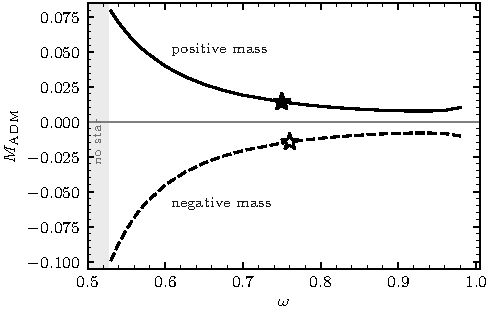
\includegraphics{fig_family.pdf}
\caption{ADM mass of isolated stars against the oscillation frequency $\omega$, for positive-mass (solid) and negative-mass (dashed) stars at the couplings used here. Star symbols: the two stars of the reference pair, whose $|M_{\rm ADM}|$ agree to $0.4\%$. At equal $\omega$ the negative-mass star is heavier in magnitude, and neither family has a star lighter than about $0.54$ of the reference mass.}
\label{fig:family}
\end{figure}

Figure~\ref{fig:family} shows both families. The reference pair consists of a positive-mass star at $\omega=0.750$, with $M_+=+0.014350$, and a negative-mass star at $\omega=0.7603$, with $M_-=-0.014295$. We call such a pair an equal-mass pair, since $|M_-|=M_+$ to $0.4\%$. Equal ADM masses are the relevant match because, in Bondi's point-mass limit, each body acts on the other through its exterior field, which the ADM mass sets. We write $\bar M=\tfrac12(M_++|M_-|)$ for the mean mass of a pair, $0.014322$ for the reference pair. The positive-mass star has a root-mean-square (rms) radius of $4.34$, the rms distance from its barycentre weighted by $w_s$ of Eq.~\eqref{eq:bary} below, and a compactness $M/R\sim3\times10^{-3}$, two orders of magnitude below that of any star near forming a horizon. Four isolated positive-mass stars with $\omega=0.75$ to $0.90$, evolved to $t=120$, keep their minimum lapse within $1.2\times10^{-3}$ of its initial value. Each star's conjugate momentum is set from the lapse of its own solution, $\Pi=-(\omega/\alpha(r))\,\varphi_0(r)$, so that it starts in its stationary state.

\subsection{The pair}
\label{sec:construction}

We place the two stars at $x=\pm d_0/2$ about the centre of the domain, where $d_0$ is the initial separation, and superpose their fields. \texttt{GRTresna}~\cite{grtresna} then solves the Hamiltonian and momentum constraints for the pair, with each field's sources entering with its sign. Two choices in this step matter for the measurement, and we state them because other studies of mixed-sign matter will meet them.

\emph{Both stars on the same slicing.} The CTTK method of \texttt{GRTresna}~\cite{cttk} can set the initial $K$ algebraically from the local energy density, $K\propto\sqrt{\rho}$, which is imaginary where $\rho<0$; the negative-mass star therefore requires its maximal-slicing option, $K=0$, which solves for $\psi$ instead. If the positive-mass star is built with the algebraic option, the two stars are built by different methods, and the positive-mass star starts inside a coherent contraction with $\max|K|\approx0.1$, four orders of magnitude above that of the negative-mass star. We therefore use $K=0$ for both stars. This removes the initial transient in $K$ ($\max|K|\approx10^{-5}$), and the two constructions then differ only in the sign of $\rho$.

\emph{The same grid spacing for the solve and the evolution.} The elliptic solve runs on a domain twice the size of the evolution domain. If its grid spacing differs from that of the evolution, the metric interpolated onto the evolution grid is displaced from the scalar field by a fraction of a cell, so each star starts away from the centre of its own gravitational potential. This produced a drift that did not converge away with resolution and was as large as the effect we measure. We therefore solve on the evolution's grid spacing, so that the cell centres coincide and the metric is copied cell by cell onto the evolution grid, while the scalar field is set on that grid from each star's radial profile. The offset between the centroids of the metric perturbation and of the matter is then below the diagnostic's precision of $10^{-4}$ in every simulation.

Both stars are given the same internal phase. For the mixed pair the relative phase has no effect, because the two fields do not couple. For two stars of the same field it matters: two Q-balls in phase attract each other through the shared field, and two in antiphase repel~\cite{battye_sutcliffe2000,palenzuela2008}. Our same-sign pairs therefore start in the attracting configuration, consistent with the mergers of Sec.~\ref{sec:nulls}. Superposed data for two stars of one field also carry phase-dependent constraint errors, which the constraint solve reduces but does not remove~\cite{helfer2022}; we use these pairs only as controls for the centroid motion.

\section{Numerical methods, diagnostics and tests}
\label{sec:setup}

\subsection{Evolution}

We evolve the Einstein equations in the conformal and covariant Z4 (CCZ4) formulation~\cite{alic2012} with constraint-damping parameters $(\kappa_1,\kappa_2,\kappa_3)=(3,0,1)$, $1{+}\log$ slicing~\cite{bona1995} and a Gamma-driver shift~\cite{campanelli2006,baker2006} with damping parameter $\eta=1$. Spatial derivatives use fourth-order finite differences, time integration the fourth-order Runge--Kutta method, and we add Kreiss--Oliger dissipation of strength $\sigma=2$. The CCZ4 variable $\chi=(\det\gamma_{ij})^{-1/3}$, equal to $\psi^{-4}$ on the conformally flat initial data, is below 1 in a positive-mass star and above 1 in a negative-mass star. The time step is $\Delta t=0.02\,\Delta x$, an order of magnitude below the usual CCZ4 value: it is set by the stability of the sextic self-interaction, and at $\Delta t=0.2\,\Delta x$ the star disperses. The outer boundaries use Sommerfeld conditions. Outgoing waves of a massive field reflect from boundary conditions designed for massless waves, so an absorbing layer, extra Kreiss--Oliger dissipation that rises with radius, covers $24\le r\le32$. With it, the net flux into the domain through its boundary stays below $10^{-7}$, even for the same-sign pairs.

All simulations use a uniform grid without mesh refinement, so a change of resolution is a change of the grid spacing alone. The domain is a cube of side $L=64$ with $N=128$, $192$ or $256$ cells per side ($\Delta x=0.50$, $0.33$, $0.25$), which puts about 9, 13 and 17 grid points across the rms radius of a star. One simulation doubles the side to $L=128$ at $N=256$ ($\Delta x=0.50$), with the absorbing layer at $48\le r\le60$, to extract gravitational waves at larger radii. The reference initial separation is $d_0=10$, about twice the radius that contains $90\%$ of a star's weight $w_s$; other pairs use $d_0=8$ to $20$. Every pair is released from rest, without a boost, so any motion is dynamical. Most simulations end at $t=200$; Table~\ref{tab:matrix} lists the exceptions. Each simulation ran on one NVIDIA H100 GPU; a simulation to $t=200$ takes about 1, 5 and 15 hours at $N=128$, $192$ and $256$.

\subsection{Diagnostics}

We track each field in two ways. Its barycentre
\begin{equation}
\bar x^{(s)}=\frac{\int x\,w_s\,d^3x}{\int w_s\,d^3x},\qquad w_s=\left(|\Phi_s|^2+|\Pi_s|^2\right)^{1/2},
\label{eq:bary}
\end{equation}
is computed over the whole domain, with $\Pi_s$ the conjugate momentum of $\Phi_s$. Its core position is the $w_s^4$-weighted centroid of the cells where $w_s$ exceeds a fixed fraction of its maximum, which ignores the low-amplitude field a star sheds. The main diagnostic is the midpoint of the two stars and its displacement,
\begin{equation}
X=\tfrac12\left(\bar x^{(+)}+\bar x^{(-)}\right),\qquad \Delta X(t)=X(t)-X(0),
\label{eq:mid}
\end{equation}
which Bondi's argument predicts to accelerate and which stays zero by symmetry for the same-sign controls. The two ways of tracking agree on $\Delta X$ of the mixed pair to $1\%$. The separation $d$ is the coordinate distance between the two barycentres; we also measure the proper distance between the two cores along the axis, $\int\sqrt{\gamma_{xx}}\,dx$. The acceleration $a$ is twice the quadratic coefficient of the least-squares fit
\begin{equation}
X(t)=X_0+v_0\,t+\tfrac12\,a\,t^2,\qquad 5\le t\le t_{\rm end},
\label{eq:fit}
\end{equation}
which leaves out the first five time units while the gauge adjusts. For point masses with $|M_-|=M_+$, each star is accelerated by the other's active mass, and Bondi's argument predicts
\begin{equation}
a=\frac{\bar M}{d^2}.
\label{eq:bondilaw}
\end{equation}
The matter momentum of each field and their signed total are
\begin{equation}
P^{(s)}=\int S_x[\Phi_s]\,\sqrt{\gamma}\,d^3x,\qquad P=P^{(+)}-P^{(-)},
\label{eq:momentum}
\end{equation}
with $\gamma=\det\gamma_{ij}$. We also record the $L_2$ norms of the Hamiltonian and momentum constraints over the domain, the multipoles of the Newman--Penrose scalar $\Psi_4$, which carries outgoing gravitational waves, on spheres of radius $R$, and the energy conditions. The NEC is violated only where $\Phi_-$ is nonzero, and the isolated positive-mass star satisfies it everywhere.

\begin{table*}[t]
\caption{The 34 simulations. Labels name the stars, P for a positive-mass and M for a negative-mass star, followed by the initial separation $d_0$. Unless stated, a simulation uses the stars of the reference pair ($\omega=0.750$ and $0.7603$, $|M_-|/M_+=0.996$), the domain $L=64$, and starts from rest.}
\label{tab:matrix}
\begin{ruledtabular}
\begin{tabular}{lp{0.31\textwidth}lll}
Label & Configuration & $N$ & $t_{\rm end}$ & Purpose \\
\hline
PM10 & mixed pair, $d_0=10$ & 128, 192, 256 & 200 & reference; resolution study \\
PM8, PM12, PM16, PM20 & mixed pair, $d_0=8$, 12, 16, 20 & 128 & 200 & dependence on separation \\
E0.64, E1.34, E1.57 & as PM20, both stars rebuilt with $|M_-|=M_+$ (to $0.02\%$) and $\bar M$ equal to 0.64, 1.34 and 1.57 times that of PM20 & 128 & 200 & dependence on mass \\
R0.60, R0.80, R1.33 & as PM10, one star rebuilt so that $|M_-|/M_+=0.60$, 0.80, 1.33 & 128 & 200 & unequal masses \\
MP10 & as PM10, the two stars exchanged & 128 & 200 & reversal \\
PM10-t400 & as PM10 & 128 & 400 & constancy of $a$ \\
PM10-rec & as PM10, domain recentred on the pair during the run & 128 & 784 & separation after $t=200$ \\
PM10-off & as PM10, pair started 10 units off centre in a fixed domain & 128 & 600 & separation after $t=200$ \\
PM10-tol & as PM10, elliptic-solver tolerance 4.4 times tighter & 128 & 200 & initial-data accuracy \\
PM10-AMR & as PM10, mesh refinement allowed & 128 & 200 & grid structure \\
PM10-$\eta$2 & as PM10, shift damping $\eta=2$ & 128 & 200 & gauge \\
PM10-L128 & as PM10, $L=128$ ($\Delta x=0.50$) & 256 & 200 & domain size; wave extraction \\
\hline
PP10 & two positive-mass stars, $d_0=10$ & 128, 192, 256 & 200 & same-sign control \\
MM10 & two negative-mass stars, $d_0=10$ & 128 (twice), 192 & 200 & same-sign control \\
P & isolated positive-mass star at the centre of the domain & 128 & 200 & isolated control \\
M, M-t1000 & isolated negative-mass star, 5 units off centre & 128 & 200, 1000 & isolated control \\
S0.75--S0.90 & isolated positive-mass stars with $\omega=0.75$, 0.80, 0.85, 0.90 & 128 & 120 & stationarity of the stars \\
\end{tabular}
\end{ruledtabular}
\end{table*}

\subsection{Tests}
\label{sec:tests}

Bondi's argument makes five predictions for a mixed pair with $|M_-|=M_+$, and each has a control:
(i)~the midpoint $X$ accelerates at a constant rate while the separation $d$ stays constant;
(ii)~the signed matter momentum $P$ stays zero while the momentum of each field grows;
(iii)~the acceleration follows Eq.~\eqref{eq:bondilaw}, $a\propto d^{-2}$ at fixed mass and $a\propto\bar M$ at fixed separation, and each star responds to its partner's mass;
(iv)~exchanging the two stars reverses the acceleration;
(v)~pairs without a mass dipole, the same-sign pairs and the isolated stars, do not move their centroids.
A numerical artefact would fail at least one of these tests: it need not reverse when the stars are exchanged, need not follow $d^{-2}$ or the partner's mass, and would also appear in the controls. Section~\ref{sec:results} takes the tests in turn.

\begin{figure*}[t]
\centering
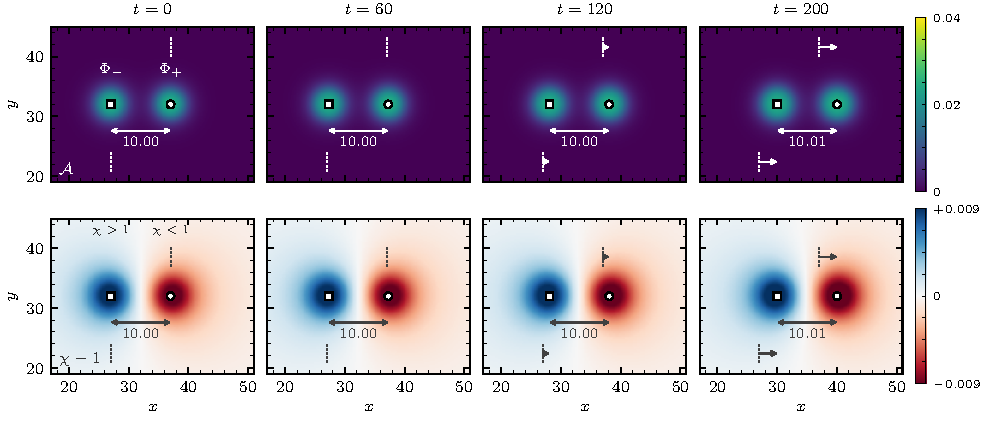
\includegraphics{fig_chase_frames.pdf}
\caption{The runaway in the headline cell (\texttt{PM}, $d_0=10$, $\Delta x=0.25$), $z=0$ plane, at $t=0$, $60$, $120$, $200$. Top: scalar-field activity $\mathcal{A}=\sum_s(|\Phi_s|^2+|\Pi_s|^2)^{1/2}$, both sectors, projected. Bottom: $\chi-1$; the phantom star is a \emph{hill} ($\chi>1$, blue, left) and the canonical star a \emph{well} ($\chi<1$, red, right)---the model's one sign made visible. Colour bars are locked across stills. Open markers: the tracked cores (circle $\Phi_+$, square $\Phi_-$); dashed ticks: release positions; arrows: displacement since release; bracketed number: the measured gap. Both stars move toward $+x$ at constant acceleration while the gap holds to $1\%$. Movie: Video~1; \href{https://youtu.be/egzPDbz2_B0}{\nolinkurl{youtu.be/egzPDbz2_B0}}.}
\label{fig:frames}
\end{figure*}

\begin{figure*}[t]
\centering
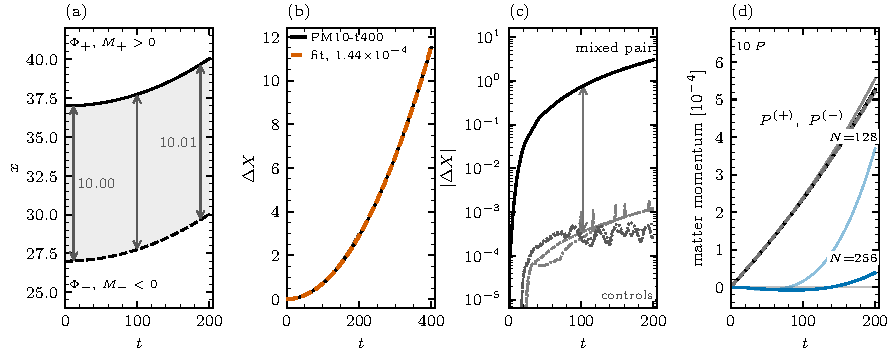
\includegraphics{fig_trajectories.pdf}
\caption{(a)~Core worldlines in the headline cell ($\Delta x=0.25$): the phantom chases the canonical star it repels; the gap is marked at three times. (b)~Midpoint drift of the $t=400$ run (solid) with the single constant-acceleration fit over $5\le t\le400$ (orange dashed)---one parabola holds for the whole run---and the finest-grid $t\le200$ cell (dashed). (c)~The signal against every null on a log scale: the mixed pair's midpoint displacement over the lone stars' core drift and the same-sign pairs' \emph{centroid} displacement (those stars merge; their centroids stay below $8\times10^{-4}$, Fig.~\ref{fig:samesign}b)---$225\times$ above the like-for-like barycentre floor, ${\sim}2000\times$ above the cores (Sec.~\ref{sec:nulls}). (d)~The Bondi signature itself: each sector's volume-integrated matter momentum climbs to ${\sim}5\times10^{-4}$ while the \emph{signed} sum of Eq.~\eqref{eq:adm_sources} (blue, magnified ten times) holds at zero---and holds better on the finer grid, the base rung being the fainter curve. Displacement without momentum, measured. $t=400$ movie: Video~2; \href{https://youtu.be/zZcr2N12aww}{\nolinkurl{youtu.be/zZcr2N12aww}}.}
\label{fig:traj}
\end{figure*}

\section{Results}
\label{sec:results}

\subsection{The runaway: constant rate, zero momentum, constant separation}
\label{sec:runaway}

Released at rest with the canonical star at $x=37$ and the phantom at $x=27$, \textbf{both stars accelerate toward $+x$ as a unit} (Figs.~\ref{fig:frames} and \ref{fig:traj}). On the finest grid the midpoint moves $\Delta X=+3.0016$ by $t=200$ at fitted acceleration $a=1.549\times10^{-4}$; a single parabola fits the whole trajectory. The $t=400$ run (base grid, where $a=1.45\times10^{-4}$) shows the rate is \emph{sustained}: fitted over $[133,266]$, $[300,400]$ and $[350,400]$ the acceleration is $1.451$, $1.422$ and $1.417\times10^{-4}$---steady to $2\%$ across a factor three in elapsed time, with the pair at $0.056c$ and still gaining speed linearly when the run ends. There is no impulse, no saturation, and no secondary acceleration.

The two Bondi signatures frame that motion. \textbf{Displacement without momentum} (Fig.~\ref{fig:traj}d): each sector's volume-integrated momentum grows steadily---both reach $5.3\times10^{-4}$ by $t=200$, the scale set by $M|v|$---while the \emph{signed} total of Eq.~\eqref{eq:adm_sources} cancels to $3.8\times10^{-6}$, under $1\%$ of either term, and that residual \emph{converges toward zero} with the grid ($3.7\times10^{-5}$ at $N=128$, $3.8\times10^{-6}$ at $N=256$), so it is a discretization residual and not a floor. (The cancelling quantity is the matter momentum of Eq.~\eqref{eq:adm_sources}, not the ADM momentum---a distinction without numerical consequence at compactness $M/R\sim3\times10^{-3}$.) The pair moves three units while carrying no net momentum, exactly as the signed bookkeeping demands. \textbf{Constant separation:} the barycentre gap ends at $9.915$ and the core gap at $10.013$, and the \emph{proper} separation between the cores, $\int\!\sqrt{\gamma_{xx}}\,dx$ along the axis, runs $10.0001\rightarrow10.0244$---so rigidity holds to $1\%$ over $t\le200$ whether it is read in coordinates or in proper distance (the long run opens the gap late, and does so in proper distance too; Sec.~\ref{sec:caveats}).

The matter survives the acceleration. The field peak is flat to $0.3\%$ over the run, the sector rms radii grow only from $4.3$ to $\sim\!5.2$, the minimum lapse never leaves $0.991$, and $\min\chi=0.9889$---nowhere near collapse ($\chi\to0$) or dispersal. A lone star under the same numerics holds its peak to $0.5\%$ for $t=200$.

\subsection{The force law: $a\,d^2$ returns the stars' mass}
\label{sec:forcelaw}

\begin{figure}[t]
\centering
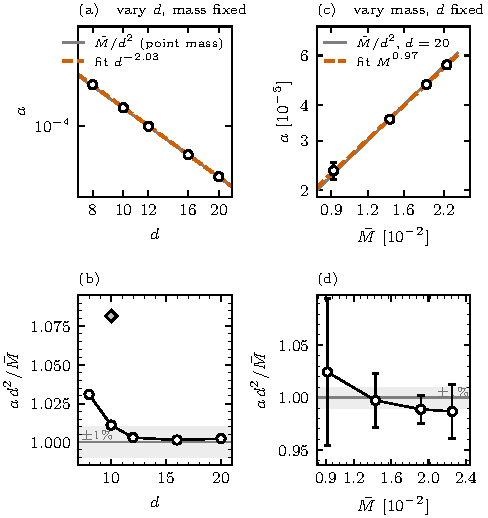
\includegraphics{fig_forcelaw.pdf}
\caption{Both axes of $a=\bar M/d^2$, measured. \emph{Left, mass fixed:} (a)~fitted acceleration against separation over $d_0=8$--$20$ at the base grid (open circles); the power-law fit (orange dashed) gives $d^{-2.03\pm0.01}$, and the point-mass line $\bar M/d^2$ (grey) is indistinguishable from it at this scale. (b)~$a\,d^2$ over the pair mass $\bar M$: the close-pair excess decays monotonically, gone by $d=16$. The open diamond is the converged ($N=256$) value at $d=10$; the ${\sim}7\%$ base-grid calibration is common to the scan and cancels from the exponent and the trend (Sec.~\ref{sec:convergence}). \emph{Right, separation fixed:} (c)~the equal-mass ladder at $d_0=20$---four pairs whose \emph{two} stars are retuned together, spanning a factor $2.46$ in mass---returns $a\propto\bar M^{0.97\pm0.06}$ against $1$ exact. (d)~The same ladder compensated: each rung recovers its own mass to within $2.4\%$, and the residual tilt carries the finite-size sign, the lightest pair being the most diffuse. Error bars are the half-spread of four disjoint-window fits. The ladder is fitted on the halo-free core tracker; the barycentre alternative is quantified in Sec.~\ref{sec:forcelaw}.}
\label{fig:forcelaw}
\end{figure}


Bondi's law is quantitative: each star is accelerated by the \emph{other's} active mass, so $a=\bar M/d^2$. Five separations test it (Fig.~\ref{fig:forcelaw}a,b). A power law through the five accelerations gives \textbf{$a\propto d^{-2.028\pm0.011}$} against $-2$ exact---and adding the widest point moved the exponent \emph{toward} the exact value (four-point fit: $-2.041$). The normalization is the stars' own mass: across the scan, $a\,d^2/\bar M=1.031\rightarrow1.011\rightarrow1.003\rightarrow1.001\rightarrow1.002$. The close-pair excess is physical and behaves like the finite-size correction it must be---largest exactly where the two stars' envelopes overlap most, decaying monotonically, gone by $d=16$. The $d=20$ cell rules out a measurement floor---$a\,d^2$ does not plateau---and the signed residual momentum halves with each step outward too ($5.8$, $3.7$, $2.3$, $0.98$, $0.49$ in units of $10^{-5}$ at $t=200$), tracking the acceleration rather than a diagnostic floor.

One systematic spans the whole scan: all five points share the base grid, whose acceleration at $d=10$ sits ${\sim}7\%$ below the converged fine-grid value (next subsection). The calibration is common mode and cancels from the exponent, from the trend in $a\,d^2$ and from every ratio in Sec.~\ref{sec:scaling}, but the \emph{absolute} accelerations---$2.307$, $1.448$, $0.998$, $0.560$, $0.359$ in units of $10^{-4}$---carry a grid uncertainty of that size: the converged $d=10$ acceleration, $(1.55\pm0.01)\times10^{-4}$, lands $8\%$ above $\bar M/d^2$, so at a gap of two stellar diameters the point-mass formula holds to ten percent rather than one. A converged separation scan is the natural sequel.

The law's other axis is the mass. Three further pairs were built at $d_0=20$---far enough out that the excess of Fig.~\ref{fig:forcelaw}b has decayed to $0.2\%$---with \emph{both} stars retuned together, so each pair stays mass-matched and therefore rigid; an unequal pair deforms (Sec.~\ref{sec:scaling}), and a quadratic fit to a moving separation measures nothing. Equal masses need \emph{different} frequencies in the two sectors (Fig.~\ref{fig:family}), so each phantom partner was root-found on its branch. With the archived $d_0=20$ cell as the fourth rung the ladder spans a factor $2.46$ and returns \textbf{$a\propto\bar M^{0.966\pm0.061}$}, $0.6\sigma$ from unity, each rung's own $a\,d^2/\bar M$ landing within $2.4\%$ of $1$ (mean $0.999$) with the residual tilt carrying the finite-size sign (Fig.~\ref{fig:forcelaw}c,d). The exponent is quoted on the halo-free core tracker; on whole-domain barycentres it returns $1.17\pm0.08$---the lightest, most diffuse rung sheds the most halo and its barycentre fit sits $18\%$ low---so the two trackers bracket the exact law. Both axes of $a=\bar M/d^2$ are therefore direct measurements---and this one is compared rung by rung against its own prediction, not against a neighbour.

\subsection{Convergence, and what cannot move the answer}
\label{sec:convergence}

\begin{figure*}[t]
\centering
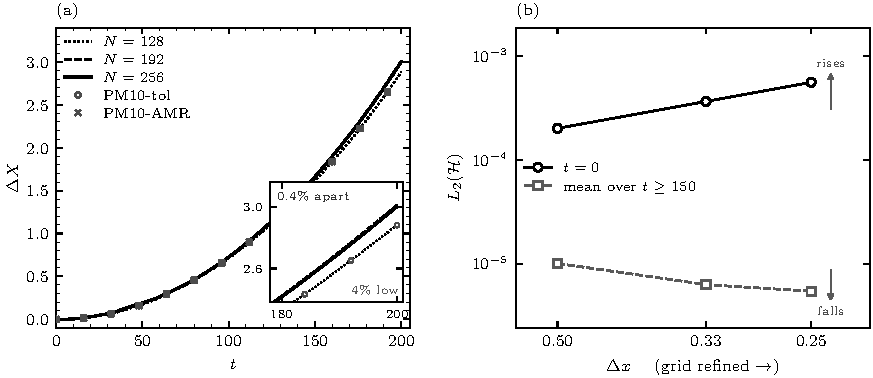
\includegraphics{fig_convergence.pdf}
\caption{(a)~The resolution ladder at $d_0=10$: midpoint drift at $\Delta x=0.50$, $0.33$, $0.25$, with two twins of the base rung overlaid---the elliptic solve driven $4.4\times$ deeper (circles) and mesh refinement enabled (crosses); both reproduce it to $2\times10^{-5}$. Inset: the endpoint---the two fine grids agree to $0.4\%$ while the base rung sits $4\%$ low. (b)~Two competing error sources: the $t=0$ violation \emph{rises} with resolution (the solve-to-evolution transfer residual, amplified as $\Delta x^{-2}$; Appendix~\ref{app:constraints}) while the evolution's own \emph{falls}---two opposite grid behaviours never leave a single asymptotic power.}
\label{fig:convergence}
\end{figure*}

Refining the grid does not erode the runaway---it settles it. The drift at $t=200$ runs $+2.881$, $+3.014$, $+3.002$ down the ladder: the two fine rungs agree to $0.4\%$ on drift and $0.5\%$ on acceleration while the base rung sits $4\%$ low, which is the opposite of what a discretization artefact does. \textbf{We quote $\Delta X(200)=3.00\pm0.01$ and $a=(1.55\pm0.01)\times10^{-4}$}, the fine-pair spread as the error bar. No formal convergence order accompanies this, for a measured reason (Fig.~\ref{fig:convergence}b): the $t=0$ Hamiltonian norm \emph{rises} with resolution ($2.0\rightarrow3.7\rightarrow5.6\times10^{-4}$, the transfer residual of Appendix~\ref{app:constraints}) while the evolution error falls ($1.0\times10^{-5}\rightarrow5.4\times10^{-6}$ late-time), so the triple is non-monotone and Richardson extrapolation would return corrections smaller than the fine-pair spread at any assumed order.

Twins of the base rung close the remaining loopholes. First, the base rung is not solve-limited: a cell identical except for the elliptic tolerance---driven from $8.6\times10^{-4}\%$ to $1.9\times10^{-4}\%$, a $4.4\times$ deeper residual---changes the drift by $0.0015\%$ and the acceleration by less than a part in $10^4$, while refining the grid moves it by $4\%$; the rung offset is a property of the evolution grid, not of the solve. Second, the uniform-grid choice does not shape the result: the same cell with mesh refinement enabled reproduces drift and acceleration to $0.001\%$--$0.002\%$, and level~1 was never created, the tagger's threshold ($|\chi-1|=0.02$) sitting four times above anything these spacetimes produce. Third, neither does the gauge: doubling the Gamma-driver damping ($\eta=1\to2$), one parameter and nothing else, shrinks the shift by $5.0\%$ everywhere while the drift moves by $0.007\%$ and the acceleration by $0.019\%$---the coordinates changed by three hundred times more than the physics did. Finally, doubling the box (eight times the volume, sponge moved out) changes the drift by $-4.2\%$: the boundary is not driving the motion.

\subsection{The mirror: swap the sectors, the runaway reverses exactly}
\label{sec:mirror}

Swapping the two sectors in place must reverse the physics and nothing else. \textbf{It reverses to two parts in $10^5$}: the mirrored cell returns drift ratio $-1.000022$ and acceleration ratio $-1.000010$ against the headline cell. What that excludes is precise: any asymmetry of the machinery that is \emph{not} sourced by the matter---a biased stencil, a lopsided box, a directional diagnostic---since none of those knows which star carries the minus sign. It does not exclude a matter-sourced artefact, which reverses under the swap just as the physics does; the retired displaced-initial-data artefact of Sec.~\ref{sec:construction} would have passed this test. Those are excluded instead by the force law, the mass ladder and the nulls that follow.

\subsection{The nulls, and the two interaction channels}
\label{sec:nulls}

\begin{figure}[t]
\centering
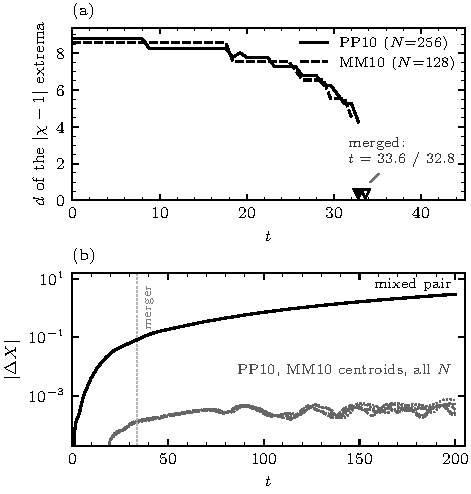
\includegraphics{fig_samesign.pdf}
\caption{The same-sign controls. (a)~Gap between the two $|\chi-1|$ extrema---wells for \texttt{PP}, hills for \texttt{MM}---tracked frame by frame: \emph{both} pairs fall together and merge, at $t=33.6$ and $32.8$. Newtonian gravity's sign is \emph{opposite} between these two cells, so their common clock is set by the sign-blind shared-field attraction, ${\sim}35\times$ gravity at this gap---a channel the mixed pair structurally lacks. (b)~Through plunge, merger and ringdown, the \texttt{PP}/\texttt{MM} pair centroids (all grids) stay below $8\times10^{-4}$---four orders under the mixed pair's drift. Movies: Videos~3 \href{https://youtu.be/jsp-Tv-f68Y}{\nolinkurl{youtu.be/jsp-Tv-f68Y}} and~4 \href{https://youtu.be/_J8jfzUk-m4}{\nolinkurl{youtu.be/_J8jfzUk-m4}}.}
\label{fig:samesign}
\end{figure}

The lone-star rows calibrate the floor: a single star, alone in the box, moves at most $1.8\times10^{-3}$ on any axis in $t=200$ (canonical, box centre) and $1.6\times10^{-3}$ (phantom, released \emph{off-centre} at $x=37$, where no symmetry protects it)---about $2000\times$ below the signal, with no preferred direction. The pair drift is measured on barycentres, so the like-for-like floor is the phantom's own barycentre: $1.3\times10^{-2}$ over the same window, a factor $225$ below the signal (cores alone would suggest $1600$--$2000$); both are correct for what they track, and the null rests on the smaller ratio.

The phantom was also carried alone to $t=1000$, five times the standard window. It reproduces the $t=200$ control digit for digit through their overlap, then keeps going without collapsing or dispersing---but it does not hold its amplitude indefinitely: the field peak decays \emph{linearly} at $0.632\%$ per $100$ time units from $t\approx200$ (disjoint sub-windows $0.604$, $0.648$, $0.608$), reaching $-5.4\%$ at $t=1000$. Everything else stays benign: $\min\chi$ \emph{rises} $1.00000\rightarrow1.00033$ (negative ADM mass holds $\chi$ above unity everywhere, so even the domain minimum is a hill), the rms radius grows $4.41\rightarrow4.83$, the confined fraction falls $0.736\rightarrow0.670$, and the Hamiltonian norm falls $44\times$ as the initial transient radiates. The star relaxes outward and leaks slowly; it does not go unstable. The same curve reads $-0.5\%$ at $t=200$ and $-1.6\%$ at $t=400$, which is why no shorter run resolves it---and why the claim here is a measured decay rate over the window evolved, not an asymptotic one.

The same-sign pairs are the campaign's sharpest control, and their behaviour was not anticipated: \textbf{they merge---both of them, on the same clock}. Tracked frame by frame (Fig.~\ref{fig:samesign}a), the two canonical stars of \texttt{PP} coalesce at $t=33.6$ and the two phantoms of \texttt{MM} at $t=32.8$---a $2.4\%$ difference, within the trackers' grid disparity. That timing is the measurement. Newtonian gravity \emph{attracts} the \texttt{PP} pair and \emph{repels} the \texttt{MM} pair---Bondi's own sign rules, Fig.~\ref{fig:schematic}---so if gravity set the timescale, \texttt{PP} would coalesce while \texttt{MM} flew apart. Instead both collapse identically: the driving force is blind to the sign of the mass, and its scale gives it away---Newtonian free fall from $d=10$ at these masses takes $t\approx207$, so the observed $t\approx33$ needs a force ${\sim}35$--$40\times$ gravity. That is the same-field overlap attraction of Sec.~\ref{sec:model}, present exactly and only where two lumps share one complex field; Bondi's $--$ repulsion is real but invisible beneath it. The pairs are seeded in phase, the attracting configuration (Sec.~\ref{sec:construction}), which is what allows them to fuse into a single centred lump.

This measurement is what certifies the mixed pair as gravitational. Its two stars are \emph{different} fields with no coupling term, so the overlap channel is structurally absent, and the data confirm that absence three ways. At the same $d=10$ where same-field pairs close in $t\approx33$, the mixed gap holds to $1\%$ for $t=200$: a few-percent leak of a $35\times$-gravity force across sectors would have closed it visibly. The mixed force is a clean $d^{-2.03}$ power law across $d=8$--$20$, where a field-overlap force dies exponentially with distance. And its strength tracks the partner's \emph{ADM mass} (next subsection), a quantity a field force knows nothing about.

Meanwhile the same-sign cells deliver their null under the most violent history in the campaign: through plunge, merger, sevenfold ejecta growth and ringdown, their pair centroids never move more than $7.8\times10^{-4}$ (\texttt{PP}) and $5.3\times10^{-4}$ (\texttt{MM}) on any of six cells across three grids (Fig.~\ref{fig:samesign}b)---and the residual does not grow with resolution. Neither pair has a mass dipole, so neither centroid moves, \emph{even during a merger}. The merger dynamics themselves are converged physics (ejecta growth $\times7.1/7.0/6.9$ across the ladder), and the remnants carry the model's structural sign difference: the \texttt{PP} remnant is a well in $\chi$ ($\min\chi=0.979$), the \texttt{MM} remnant a \emph{hill} ($\chi$ up to $1.011$)---same matter behaviour, opposite curvature.

\subsection{Gravity scales with the source, and the gap's sign flips at equal mass}
\label{sec:scaling}

\begin{figure}[t]
\centering
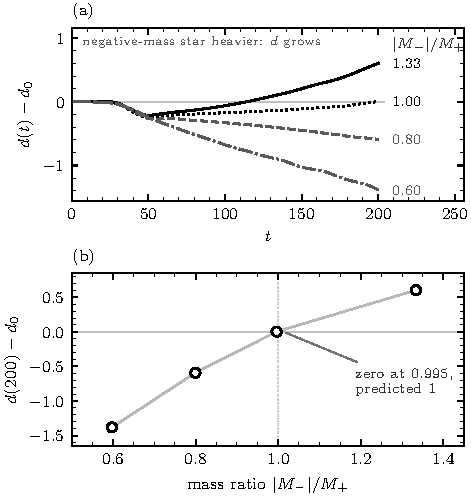
\includegraphics{fig_massscale.pdf}
\caption{The mass ladder: the matched pair and three retuned partners spanning a factor $2.2$ in mass ratio. (a)~Gap history: with a heavier phantom the gap \emph{opens}, matched it holds, with a lighter phantom it \emph{closes}, monotonically in the ratio. Every cell shares the same $t\approx50$ gauge dip, so the gap is read late. (b)~Gap change at $t=200$ against the pair mass ratio $|M_-|/M_+=0.597$, $0.800$, $0.996$, $1.333$, monotone through the four cells: the sign flip falls at ratio $0.995$, against $1.000$ predicted.}
\label{fig:massscale}
\end{figure}


Each star is accelerated by the \emph{other's} mass, so retuning one star must change its partner's acceleration and leave its own alone. Three one-knob variants test this (Fig.~\ref{fig:massscale}), retuning $\Phi_-$ to $\omega=0.88$ and $0.804$ and, for the phantom-heavier rung, the \emph{canonical} star to $\omega=0.81$. The constant $C$ in $\ddot x=\pm C/d(t)^2$ is fitted per star by regressing its core's $x(t)$ on $\{1,t,I_2(t)\}$ over $t\ge5$, where $I_2$ is the double time integral of the \emph{measured} $d(t)^{-2}$; the fit does not assume constant separation. Only ratios of $C$ are quoted, so the grid calibration of Sec.~\ref{sec:forcelaw} cancels. The absolute counterpart is the equal-mass ladder. Mass factors $0.600$, $0.803$, $0.747$ return retuned-partner pull ratios $0.618$, $0.810$, $0.756$---within $0.9$--$3.1\%$ across a factor $2.2$---with unchanged-partner controls $1.028$, $1.011$, $1.001$. No rung exists below $0.60$ of the matched mass: both branches floor at $|M|_{\min}\simeq0.54$ of it (Fig.~\ref{fig:family}), which is itself a result. And the ladder carries a signature with no artefact analogue: \textbf{the gap's behaviour flips sign exactly where the masses cross}. Heavier phantom: the gap opens ($+0.60$). Matched: it holds ($+0.003$). Lighter phantom: it closes ($-0.59$, $-1.38$), monotonically. Interpolating between the two cells that bracket the flip puts it at mass ratio $0.995\pm0.03$, against $1.000$ predicted; the error bar is the spread over end-of-run gap conventions (barycentre $0.995$, proper $0.994$, core $0.961$, late-window mean $1.002$), which dominates the statistical one. No grid, boundary or solver distinguishes which of the two stars is heavier; gravity does.

\section{Limits on gravitational radiation and near-zone behaviour}
\label{sec:weyl}

A uniquely relativistic aspect of the runaway is its radiation: the exact accelerating-pair metrics are radiative~\cite{bonnor_swami1964,bicak1983}, and negative-mass binaries have been proposed as sources of anomalous signatures~\cite{trivedi_loeb2026}, with the leading anomalous channel for mismatched charge-to-inertia binaries being dipolar. The bicomplex model closes that channel structurally: the source of gravity is the signed stress tensor, conserved on shell (Sec.~\ref{sec:model}), so the rate of change of the signed mass dipole is the conserved signed momentum---zero for this data, and measured to cancel to $\lesssim1\%$ (Sec.~\ref{sec:runaway})---and mass-dipole radiation is forbidden at leading order for exactly the reason it is forbidden in ordinary general relativity. Kinematics agrees from the other side: $\Psi_4$ carries spin weight $-2$, so its expansion begins at $\ell=2$ whatever the dipole does. What survives is quadrupolar bremsstrahlung from the accelerating pair---secular, chirpless, and for this configuration very small. The signed mass quadrupole of a zero-momentum pair is $Q\simeq2\bar M d\,X(t)$, so at constant separation and constant acceleration $\ddot Q=2\bar M a d$ is \emph{constant}: measured at $4.5\times10^{-5}$ against $4.4\times10^{-5}$ predicted, steady to $7\%$ over $20\le t\le190$. A constant $\ddot Q$ radiates nothing at leading order, and the flux enters only through the slow secular evolution of $d$ and $v$---from the trajectories $|\dddot Q|\le6\times10^{-8}$, a quadrupole luminosity ${\sim}4\times10^{-17}$ and ${\sim}7\times10^{-15}$ radiated over the run, ten orders of magnitude below the pair's total mass of $5.5\times10^{-5}$. So the $\ell=2$ content is bounded rather than measured here, every extraction shell the domain affords lying inside the near zone.

\begin{figure}[t]
\centering
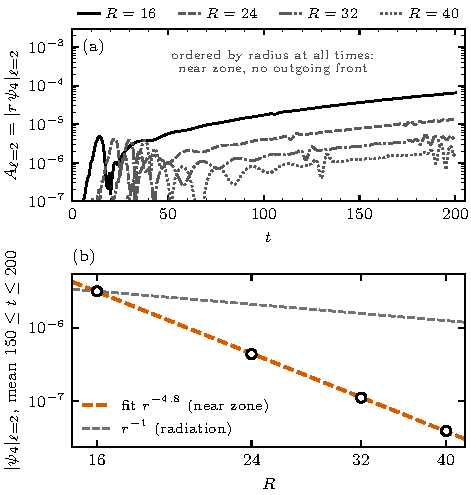
\includegraphics{fig_wavezone.pdf}
\caption{The wave-zone measurement on the doubled box ($L=128$, $\Delta x=0.25$, sponge at $48$--$60$). (a)~Total $\ell=2$ amplitude $A_{\ell=2}$ on the four extraction shells: ordered by radius at all times, with no propagating front. (b)~The falloff, averaged over $150\le t\le200$: $|\psi_4|_{\ell=2}\propto r^{-4.8}$, against $r^{-1}$ for radiation. Every shell out to $R=40$ is in the near zone, so $A_{\ell=2}$ is a Coulombic near-field amplitude, not a radiated flux---consistent with the quadrupole estimate of Sec.~\ref{sec:weyl}, ten orders of magnitude below this bound.}
\label{fig:wavezone}
\end{figure}

The doubled box measures how much of that reaches the wave zone at these speeds: \textbf{none that we can detect out to $R=40$} (Fig.~\ref{fig:wavezone}). The $\ell=2$ amplitude falls as $r^{-4.8}$ across shells spanning $R=16$--$40$---$r\,\psi_4$ drops by a factor $31$ where one outgoing wave would keep it flat---so every shell sits in the near zone, reading the source's Coulombic curvature rather than a flux. This is a null with a number, and it agrees with the structural argument above; reaching the radiative regime needs relativistic speed---only $0.03c$ inside the fit window here (Sec.~\ref{sec:discussion}).

\section{Systematics, with their measured sizes}
\label{sec:caveats}

\emph{How accelerations are measured.} Every quoted acceleration is a parabola fit to the midpoint trajectory from $t=5$ (Appendix~\ref{app:constraints}) to the end of the run. Fitting only the last two thirds of a run instead changes any single $a$ by $1$--$3\%$; the trends---the $d^{-2}$ exponent, the mass-law ratios, the sign flip at equal mass---do not change.

\emph{Grid calibration.} The base grid underestimates the acceleration by ${\sim}7\%$ at $d_0=10$; the two fine grids agree to $0.5\%$ and set the quoted values. The base-grid scans all carry the same offset, which cancels from their ratios and exponents (Sec.~\ref{sec:forcelaw}).

\emph{The gap opens after $t=200$, and why.} Over $t\le200$ the separation holds to $1\%$ (the two trackers bracket its change between $-0.9\%$ and $+0.1\%$). On the base grid it then opens: $d=11.8$ at $t=400$, $18.2$ at $t=600$, $29.8$ at $t=784$, growing roughly as $(t-t_0)^{2.8}$ with $t_0\simeq110$. What opens it is one star. The trailing phantom's acceleration falls steadily, reaches zero near $t\approx530$ and reverses, standing at $-7.5\times10^{-5}$ by $t=750$ while the leading star still accelerates at $+1.1\times10^{-4}$. \textbf{After $t\approx500$ this is one runaway star with a slowing companion, not a pair}, and no pair quantity is quoted beyond that point. (The common motion still obeys the force law: $a\,d^2$ stays within $35\%$ of $\bar M$ over the whole run while $a$ falls ninefold.)

The separation is fragile for a structural reason. With matched masses both stars accelerate equally at \emph{every} separation ($\ddot x_+=|M_-|/d^2$, $\ddot x_-=M_+/d^2$), so nothing pulls $d$ back toward $d_0$: any small difference between the two accelerations, from any source, grows without limit, while the midpoint drift that measures the runaway is unaffected. Three sources were tested. \emph{Unequal masses---no.} Three of the four equal-mass pairs are matched to better than $0.02\%$ and still open by $+0.009$ to $+0.030$ at $t=200$; the headline pair's own $0.39\%$ mismatch has the wrong sign (it would close the gap by $0.011$; the converged rung opens by $+0.013$). \emph{The moving box---no.} A recentring box run to $t=784$ and a static box started ten units off centre agree on the separation to $0.5\%$ through $t=500$ and on their field contents to $0.1\%$; the comparison stops at $t=500$ because the static box's leading star reaches the sponge at $t=600$. \emph{The grid---yes.} The opening at $t=200$ falls from $+0.107$ to $+0.029$ to $+0.013$ as $\Delta x$ goes from $0.50$ to $0.25$, an $8.4$-fold drop for a factor two in spacing: it converges away, as a physical separation change would not. At fixed grid it scales as $\bar M^{1.3}$ and $d^{-2.9}$, like a field gradient across the star ($M/d^3$) rather than the force ($M/d^2$). A plausible seed is that the discretized stars are not exactly stationary---their field content grows by $21.0$, $16.1$ and $12.4\%$ by $t=200$ down the ladder, and by the same $20.0$ and $20.9\%$ for the lone stars---and the two sectors need not drift identically; we record this as a candidate, not a demonstrated mechanism.

What follows is limited. The $t\le200$ results are unaffected: they are quoted at the converged rung, where the opening is $0.13\%$. Beyond $t=200$ the base-grid separation is unconverged, and the grid-error attribution is an extrapolation---from an opening of $0.107$, where the ladder was measured, to $8.2$ at $t=600$, a factor $77$---so no quantitative conclusion is drawn from it. One late-time run at $N=192$ would decide it; the prediction it must meet is $d(400)\simeq10.7$, against $11.85$ on the base grid. The speeds reached in the long cells---the leading star at $0.10c$ near $t=600$ and $0.12c$ at $t=784$, the midpoint at $0.081c$---come only after rigidity is gone. Relativistic speed needs a finer grid, not a longer run.

\emph{Gauge.} Drift and gap are coordinate quantities, so the gauge is checked directly. The shift at the two cores never exceeds $7.7\times10^{-4}$ and is nearly antisymmetric ($\beta^x$ points one way at the canonical star and the other at the phantom), so its mean---the only part that could move the pair as a whole---stays below $1.1\times10^{-5}$ against a midpoint velocity of $3.0\times10^{-2}$; integrated over the run it accounts for $4.0\times10^{-4}$ of displacement, $0.013\%$ of $\Delta X=3.00$. The drift is matter moving through the Eulerian frame, anchored at the Sommerfeld boundary, not coordinates being dragged; the $\eta=2$ twin of Sec.~\ref{sec:convergence} confirms it by run. Nulls are quoted on cores because a whole-domain barycentre picks up domain noise (the off-centre lone phantom's wobbles by $4\times10^{-2}$ early while its core never moves more than $1.6\times10^{-3}$); the pair is quoted on both trackers, which agree to $1\%$.

\emph{Same-sign initial data.} The conformally flat outer boundary condition of the elliptic solve is wrong for a box carrying net mass $2M$, so the same-sign solves floor near $10^{-3}\%$ instead of converging further. This is a $t=0$ statement only---their evolution constraints stay bounded through the merger---and is why those cells serve as momentum nulls, not precision measurements.

\section{Discussion and conclusion}
\label{sec:discussion}

We posed Bondi's positive--negative mass pair as a full initial-value problem, and it behaved as he argued in 1957---quantitatively.

\textbf{(1) The runaway is real, and it is steady.} Released at rest, the mixed pair self-accelerates at a rate flat to $2\%$ through $t=400$, reaching $0.056c$; at the base grid the rate eventually falls as discretization error spreads the pair, and $a\,d^2$ goes on tracking $\bar M$ in the pair's common mode, though not in the differential mode that opens the gap; rigidity is not quoted past $t\approx500$ (Sec.~\ref{sec:caveats}). Swapping the sectors reverses the drift to two parts in $10^5$; the separation holds to $1\%$ over $t\le200$, in proper distance as in coordinates.

\textbf{(2) It is gravity.} By construction the sectors meet only in the metric; by measurement the force falls as $d^{-2.03\pm0.01}$ with $a\,d^2$ returning the stars' mass, and on a mass-matched ladder spanning a factor $2.46$ the mass exponent itself comes back as $0.97\pm0.06$; differentially, the pull tracks the partner's ADM mass through a factor $2.2$---including the gap's sign flip at equal mass. The same-sign controls isolate the model's only other channel, the shared-field overlap attraction, and show it ${\sim}35\times$ gravity, short-range and sign-blind---present where the model puts it, absent from the mixed pair.

\textbf{(3) Displacement without momentum---the Bondi signature.} The sector momenta, each growing to $5\times10^{-4}$, cancel in the signed sum to under $1\%$, the residual converging \emph{toward} zero with resolution while the displacement converges onto $3.00\pm0.01$. Same-sign pairs, having no mass dipole, hold their centroids at the $10^{-4}$ level \emph{even while merging}.

\textbf{(4) It does not detectably radiate, as predicted.} The signed dipole cannot radiate---its rate of change is the conserved signed momentum---and the constant-$\ddot Q$ quadrupole radiates nothing at leading order: an estimated $7\times10^{-15}$ over the run, with the measured $\ell=2$ amplitude falling as $r^{-4.8}$ out to $R=40$---near field, not flux (Sec.~\ref{sec:weyl}).

\textbf{(5) A star of negative ADM mass exists} as constraint-satisfying, asymptotically flat initial data, and survives evolution---$400$ units paired, $1000$ alone, its peak flat to $0.5\%$ over the standard $t\le200$ window (static phantom-field stars~\cite{dzhunushaliev2014} and de Sitter bubbles~\cite{mbarek2014} were known; a negative-mass \emph{horizon} is a different object~\cite{mann1997}). It is the better-behaved of the pair, shed field being pushed away rather than re-accreted. Alone to $t=1000$ it neither collapses nor disperses but relaxes outward, its central amplitude falling linearly at $0.63\%$ per $100$ time units: a measured decay rate over the window evolved, not asymptotic stability.

\textbf{What is not established.} Four things remain open. (i)~The absolute strength of the force away from $d=10$: the separation scan ran only at the base grid, which reads ${\sim}7\%$ low (Sec.~\ref{sec:caveats}), so the exponent is secure but the normalization elsewhere is not. (ii)~Rigidity past $t=200$: on the base grid the trailing star slows and the gap opens. Every test in Sec.~\ref{sec:caveats} points to a grid error that shrinks with resolution, acting on a separation that nothing restores---but that is extrapolated a factor $77$ beyond where the resolution ladder was measured, and a late-time run at $N=192$ would decide it. (iii)~Stability against sideways perturbations: every release here is head-on. (iv)~The radiation. The near-zone null agrees with the no-dipole argument and the quadrupole estimate of Sec.~\ref{sec:weyl}, but the question this configuration was built to reach---what happens to the energy of a radiating system whose total mass is only $5.5\times10^{-5}$, $0.4\%$ of either star, with no positive-mass theorem to stop it falling---needs relativistic speed, and speed is now limited by resolution, not run time: ${\sim}0.3c$, where the anomalous-signature programme of Ref.~\cite{trivedi_loeb2026} meets a concrete source, is a converged-grid measurement waiting to be made. Nothing here bears on whether such matter exists.

\section{Reproducibility}
\label{sec:repro}

Every number and figure derives from the packed campaign under \texttt{results/bondi-dipole-runaway} of the repository~\cite{repo}: one directory per cell under \texttt{campaign/}, each holding the tracker streams, constraint norms, Weyl modes, solver history, and the exact launch environment. Cell names carry the configuration (\texttt{runaway\_pair\_d10\_L64\_N256\_lev0}: the mixed pair at $d_0=10$, $L=64$, $256^3$, uniform), and \texttt{stars/} holds the dressed-star profile tables and both family scans. A single script (\texttt{article\_figures.py}, in the repository's visualisation package) regenerates every figure and prints every quoted number. The code lives in the same repository~\cite{repo}, tagged at the version behind this paper; an archived snapshot with a DOI accompanies the published version. See Supplemental Material at [URL will be inserted by publisher] for movies of the headline cell (Video~1), its $t=400$ continuation (Video~2) and both same-sign controls (Videos~3 \texttt{PP} and~4 \texttt{MM}). Initial data: \texttt{GRTresna}~\cite{grtresna}; evolution: \texttt{GRTeclyn}~\cite{grteclyn,amrex,grchombo}.

\begin{acknowledgments}
This work was supported by Gravity Frontiers
(\url{https://www.gravityfrontiers.org/en}), which funded the underlying
research and the development of the numerical-simulation software. The authors
acknowledge the GRTL Collaboration for \texttt{GRChombo}, \texttt{GRTresna},
and \texttt{GRTeclyn}.
\end{acknowledgments}

\appendix

\section{Constraint behaviour}
\label{app:constraints}

\emph{Initial data.} The \texttt{GRTresna}~\cite{grtresna} solves themselves are clean: every mixed-pair solve converges monotonically on the maximal-slicing path and exits under its tolerance gate, with residuals of $8.6\times10^{-4}\%$ (Hamiltonian) and $8.0\times10^{-4}\%$ (momentum) at the base grid after 13 nonlinear iterations, tightening to $8.7\times10^{-5}\%$ and $5.1\times10^{-5}\%$ on the finest rung (16 iterations). The gate scales with the grid, so a fine rung never inherits a coarse rung's residual, as it would on a fixed-tolerance ladder.

The solve is not, however, what sets the $t=0$ violation on the \emph{evolution} grid: the deep-solve twin of Sec.~\ref{sec:convergence} drove the solve $4.4\times$ deeper at fixed grid and lowered that violation by only ${\sim}1\%$ ($2.02\rightarrow2.00\times10^{-4}$). What dominates is the solve-to-evolution transfer, set by the handoff order of Sec.~\ref{sec:construction}: the handoff leaves a metric--matter mismatch at the grid scale, whose amplitude does not fall with resolution, and the constraint operator reading it is a second difference carrying $\Delta x^{-2}$. No solver tolerance touches that term; removing it would mean matching the two discretizations at the order of the constraint operator itself.

The transfer error is bounded rather than removed, and transient: a $t=0$ spike that radiates away, falling by an order of magnitude within $t\lesssim3$---faster on finer grids, as a grid-scale transient should---and settling onto its late plateau by $t\approx4$, before the $t\ge5$ fit window opens.

\emph{Evolution.} Figure~\ref{fig:constraints} shows the headline ladder in absolute code units (the domain is overwhelmingly vacuum, so relative norms are dominated by near-zero denominators). Each rung relaxes from its initial-data spike within $t\lesssim2$ and then holds nearly flat for the whole run: late-time $L_2(\mathcal{H})$ of $1.0\times10^{-5}$, $6.3\times10^{-6}$, $5.4\times10^{-6}$ down the ladder---falling with resolution while the $t=0$ spike rises, the two-error-source structure of Fig.~\ref{fig:convergence}b. The zero initial shift also emits a flat ${\sim}10^{-6}$ gauge pulse inward at $t=0$ (visible in the packed shift frames~\cite{repo}); it crosses the stars by $t\approx20$ and leaves no trace in the constraints or the fitted acceleration. The \texttt{PP} control runs a factor few above the mixed cell after its merger and stays bounded to $t=200$, its centroid null holding throughout.

\begin{figure}[!tb]
\centering
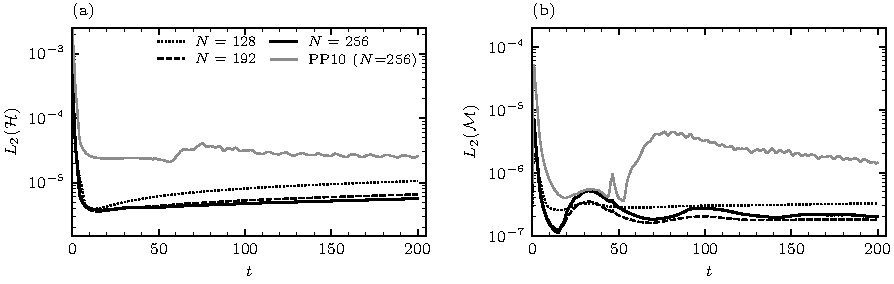
\includegraphics{fig_constraints.pdf}
\caption{Constraint norms for the headline cell's resolution ladder (line styles as in Fig.~\ref{fig:convergence}) and the merging \texttt{PP} control at the finest grid (gray). (a)~Hamiltonian, $L_2$ over the domain: finer grids start worse (initial-data interpolation noise) and evolve better. (b)~Momentum, $L_2$.}
\label{fig:constraints}
\end{figure}

\section{Computational cost}
\label{app:cost}

Every evolution ran on one NVIDIA H100 80\,GB device of a four-H100 node with two 32-core Xeon Platinum 8462Y+ processors; the elliptic solves ran CPU-side on 32 MPI ranks, ${\sim}20$ minutes at $256^3$ and ${\sim}4$ hours at $512^3$. \texttt{GRTeclyn} was built against AMReX with CUDA~12.1 and GCC~11.4; each cell's metadata records its build commit. At $\Delta t=0.02\,\Delta x$, a $t=200$ evolution takes $20\,000$/$30\,000$/$40\,000$ steps at $N=128$/$192$/$256$, using ${\sim}6$/$20$/$48$~GB of device memory (uniform $256^3$ fits on one card) and $1.1$, $4.8$--$6.0$ and $14.6$ hours of wall time, the last including the movie/still pipeline. The wave-zone box ($L=128$, $256^3$) takes $7.4$~h, the $t=400$ long run with frames $3.8$~h, the lone star to $t=1000$ $5.4$~h, and the moving-box pair to $t=784$ $4.3$~h. The thirty-four packed cells total ${\simeq}99$ GPU-hours of evolution.

\begin{thebibliography}{99}

\bibitem{bondi1957}
H.~Bondi,
\newblock ``Negative mass in general relativity,''
\newblock Rev.\ Mod.\ Phys.\ \textbf{29}, 423 (1957).

\bibitem{bonnor_swami1964}
W.~B.~Bonnor and N.~S.~Swaminarayan,
\newblock ``An exact solution for uniformly accelerated particles in general relativity,''
\newblock Z.\ Phys.\ \textbf{177}, 240 (1964).

\bibitem{bicak1983}
J.~Bi\v{c}\'ak, C.~Hoenselaers, and B.~G.~Schmidt,
\newblock ``The solutions of the Einstein equations for uniformly accelerated particles without nodal singularities,''
\newblock Proc.\ R.\ Soc.\ London A \textbf{390}, 397 (1983).

\bibitem{bonnor1989}
W.~B.~Bonnor,
\newblock ``Negative mass in general relativity,''
\newblock Gen.\ Relativ.\ Gravit.\ \textbf{21}, 1143 (1989).

\bibitem{forward1990}
R.~L.~Forward,
\newblock ``Negative matter propulsion,''
\newblock J.\ Propulsion Power \textbf{6}, 28 (1990).

\bibitem{hoffmann1966}
B.~Hoffmann,
\newblock ``Negative mass and the quasars,''
\newblock in \emph{Perspectives in Geometry and Relativity}, edited by B.~Hoffmann (Indiana University Press, Bloomington, 1966), p.~176.

\bibitem{martins1980}
R.~de~A.~Martins,
\newblock ``Causal paradoxes implied by the hypothetical coexistence of positive- and negative-mass matter,''
\newblock Lett.\ Nuovo Cimento \textbf{28}, 265 (1980).

\bibitem{caldwell2002}
R.~R.~Caldwell,
\newblock ``A phantom menace? Cosmological consequences of a dark energy component with super-negative equation of state,''
\newblock Phys.\ Lett.\ B \textbf{545}, 23 (2002).

\bibitem{morris_thorne1988}
M.~S.~Morris and K.~S.~Thorne,
\newblock ``Wormholes in spacetime and their use for interstellar travel: A tool for teaching general relativity,''
\newblock Am.\ J.\ Phys.\ \textbf{56}, 395 (1988).

\bibitem{alcubierre1994}
M.~Alcubierre,
\newblock ``The warp drive: hyper-fast travel within general relativity,''
\newblock Class.\ Quantum Grav.\ \textbf{11}, L73 (1994).

\bibitem{clough2024}
K.~Clough, T.~Dietrich, and S.~Khan,
\newblock ``What no one has seen before: gravitational waveforms from warp drive collapse,''
\newblock arXiv:2406.02466 [gr-qc] (2024).

\bibitem{mann1997}
R.~B.~Mann,
\newblock ``Black holes of negative mass,''
\newblock Class.\ Quantum Grav.\ \textbf{14}, 2927 (1997).

\bibitem{nojiri2026}
S.~Nojiri and S.~D.~Odintsov,
\newblock ``May negative mass objects exist in the sky?,''
\newblock arXiv:2602.15058 [gr-qc] (2026).

\bibitem{gleiser2006}
R.~J.~Gleiser and G.~Dotti,
\newblock ``Instability of the negative mass Schwarzschild naked singularity,''
\newblock Class.\ Quantum Grav.\ \textbf{23}, 5063 (2006).

\bibitem{shinkai2002}
H.~Shinkai and S.~A.~Hayward,
\newblock ``Fate of the first traversible wormhole: Black-hole collapse or inflationary expansion,''
\newblock Phys.\ Rev.\ D \textbf{66}, 044005 (2002).

\bibitem{friedberg1976}
R.~Friedberg, T.~D.~Lee, and A.~Sirlin,
\newblock ``Class of scalar-field soliton solutions in three space dimensions,''
\newblock Phys.\ Rev.\ D \textbf{13}, 2739 (1976).

\bibitem{coleman1985}
S.~Coleman,
\newblock ``Q-balls,''
\newblock Nucl.\ Phys.\ B \textbf{262}, 263 (1985).

\bibitem{friedberg1987}
R.~Friedberg, T.~D.~Lee, and Y.~Pang,
\newblock ``Mini-soliton stars,''
\newblock Phys.\ Rev.\ D \textbf{35}, 3658 (1987).

\bibitem{kaup1968}
D.~J.~Kaup,
\newblock ``Klein--Gordon geon,''
\newblock Phys.\ Rev.\ \textbf{172}, 1331 (1968).

\bibitem{ruffini1969}
R.~Ruffini and S.~Bonazzola,
\newblock ``Systems of self-gravitating particles in general relativity and the concept of an equation of state,''
\newblock Phys.\ Rev.\ \textbf{187}, 1767 (1969).

\bibitem{liebling2023}
S.~L.~Liebling and C.~Palenzuela,
\newblock ``Dynamical boson stars,''
\newblock Living Rev.\ Relativ.\ \textbf{26}, 1 (2023).

\bibitem{alic2012}
D.~Alic, C.~Bona-Casas, C.~Bona, L.~Rezzolla, and C.~Palenzuela,
\newblock ``Conformal and covariant formulation of the Z4 system with constraint-violating modes,''
\newblock Phys.\ Rev.\ D \textbf{85}, 064040 (2012).

\bibitem{grchombo}
T.~Andrade \emph{et al.},
\newblock ``GRChombo: an adaptable numerical relativity code for fundamental physics,''
\newblock J.\ Open Source Softw.\ \textbf{6}, 3703 (2021).

\bibitem{grteclyn}
GRTL Collaboration,
\newblock \texttt{GRTeclyn},
\newblock \url{https://github.com/GRTLCollaboration/GRTeclyn}.

\bibitem{grtresna}
J.~C.~Aurrekoetxea, S.~E.~Brady, \emph{et al.},
\newblock ``GRTresna: an open-source code to solve the initial data constraints in numerical relativity,''
\newblock arXiv:2501.13046 [gr-qc] (2025).

\bibitem{amrex}
W.~Zhang \emph{et al.},
\newblock ``AMReX: a framework for block-structured adaptive mesh refinement,''
\newblock J.\ Open Source Softw.\ \textbf{4}, 1370 (2019).

\bibitem{schoen_yau1979}
R.~Schoen and S.-T.~Yau,
\newblock ``On the proof of the positive mass conjecture in general relativity,''
\newblock Commun.\ Math.\ Phys.\ \textbf{65}, 45 (1979).

\bibitem{witten1981}
E.~Witten,
\newblock ``A new proof of the positive energy theorem,''
\newblock Commun.\ Math.\ Phys.\ \textbf{80}, 381 (1981).

\bibitem{mbarek2014}
S.~Mbarek and M.~B.~Paranjape,
\newblock ``Negative mass bubbles in de Sitter spacetime,''
\newblock Phys.\ Rev.\ D \textbf{90}, 101502(R) (2014).

\bibitem{gonzalez2009}
J.~A.~Gonz\'alez, F.~S.~Guzm\'an, and O.~Sarbach,
\newblock ``Instability of wormholes supported by a ghost scalar field. II. Nonlinear evolution,''
\newblock Class.\ Quantum Grav.\ \textbf{26}, 015011 (2009); see also \textbf{26}, 015010 (2009).

\bibitem{dzhunushaliev2014}
V.~Dzhunushaliev, V.~Folomeev, C.~Hoffmann, B.~Kleihaus, and J.~Kunz,
\newblock ``Boson stars with nontrivial topology,''
\newblock Phys.\ Rev.\ D \textbf{90}, 124038 (2014).

\bibitem{carroll2003}
S.~M.~Carroll, M.~Hoffman, and M.~Trodden,
\newblock ``Can the dark energy equation-of-state parameter $w$ be less than $-1$?,''
\newblock Phys.\ Rev.\ D \textbf{68}, 023509 (2003).

\bibitem{cline2004}
J.~M.~Cline, S.~Jeon, and G.~D.~Moore,
\newblock ``The phantom menaced: constraints on low-energy effective ghosts,''
\newblock Phys.\ Rev.\ D \textbf{70}, 043543 (2004).

\bibitem{helfer2022}
T.~Helfer, U.~Sperhake, R.~Croft, M.~Radia, B.-X.~Ge, and E.~A.~Lim,
\newblock ``Malaise and remedy of binary boson-star initial data,''
\newblock Class.\ Quantum Grav.\ \textbf{39}, 074001 (2022).

\bibitem{cttk}
J.~C.~Aurrekoetxea, K.~Clough, and E.~A.~Lim,
\newblock ``CTTK: a new method to solve the initial data constraints in numerical relativity,''
\newblock Class.\ Quantum Grav.\ \textbf{40}, 075003 (2023).

\bibitem{bona1995}
C.~Bona, J.~Mass\'o, E.~Seidel, and J.~Stela,
\newblock ``New formalism for numerical relativity,''
\newblock Phys.\ Rev.\ Lett.\ \textbf{75}, 600 (1995).

\bibitem{campanelli2006}
M.~Campanelli, C.~O.~Lousto, P.~Marronetti, and Y.~Zlochower,
\newblock ``Accurate evolutions of orbiting black-hole binaries without excision,''
\newblock Phys.\ Rev.\ Lett.\ \textbf{96}, 111101 (2006).

\bibitem{baker2006}
J.~G.~Baker, J.~Centrella, D.-I.~Choi, M.~Koppitz, and J.~van~Meter,
\newblock ``Gravitational-wave extraction from an inspiraling configuration of merging black holes,''
\newblock Phys.\ Rev.\ Lett.\ \textbf{96}, 111102 (2006).

\bibitem{trivedi_loeb2026}
O.~Trivedi and A.~Loeb,
\newblock ``Unique gravitational-wave signals from negative-mass binaries,''
\newblock arXiv:2605.10976 [gr-qc] (2026).

\bibitem{battye_sutcliffe2000}
R.~A.~Battye and P.~M.~Sutcliffe,
\newblock ``Q-ball dynamics,''
\newblock Nucl.\ Phys.\ B \textbf{590}, 329 (2000).

\bibitem{palenzuela2008}
C.~Palenzuela, L.~Lehner, and S.~L.~Liebling,
\newblock ``Orbital dynamics of binary boson star systems,''
\newblock Phys.\ Rev.\ D \textbf{77}, 044036 (2008).

\bibitem{manfredi2018}
G.~Manfredi, J.-L.~Rouet, B.~Miller, and G.~Chardin,
\newblock ``Cosmological structure formation with negative mass,''
\newblock Phys.\ Rev.\ D \textbf{98}, 023514 (2018).

\bibitem{manfredi2026}
G.~Manfredi, J.-L.~Rouet, and B.~Miller,
\newblock ``The Bondi universe: can negative mass drive the cosmological expansion?,''
\newblock arXiv:2601.22910 [gr-qc] (2026).

\bibitem{repo}
N.~M.~Shirokov,
\newblock \texttt{GRTeclyn} campaign repository (Sec.~\ref{sec:repro}),
\newblock \url{https://github.com/Nikchik-coder/GRTeclyn}.

\bibitem{shirokov2026}
N.~M.~Shirokov,
\newblock ``Wormhole dynamics: nonlinear collapse and gravitational-wave emission,''
\newblock arXiv:2604.00071 [gr-qc] (2026).

\end{thebibliography}

\end{document}
